\documentclass[11pt]{article}
\usepackage{amsmath, amssymb, amsfonts, amsthm}
\usepackage{url, graphicx}
\numberwithin{equation}{section}
\linespread{1.2}

\renewcommand{\vec}{\mathbf}
\newcommand{\mat}{\mathsf}
\title{An Introduction to Artificial Neural Networks}
\author{To be filled}
\date{24-Oct-2020}
\begin{document}
\maketitle
\section{Introduction}\label{s1}
Many inventions were inspired by observing Nature's creations. The burrs of
burdock clinging to his dress inspired George de Mestral to think of an
interlocking system of tiny threads leading him to develop Velcro. The ability
of bats to navigate in absence of light inspired people to build SONAR to
sense obstacles in deep water where light does not reach. It is, therefore,
not surprising that the human brain were the most obvious object to mimic
when people started thinking about artificial intelligence in the 1930s and 40s.
In this article, we will trace the development of artificial neural networks
since their inception in the first half of the twentieth century till today.
It is customary to begin a discussion of artificial neural networks by first
taking a glimpse of their immensely more powerful natural cousins.

The human brain has a very large number, of the order of $10^{11}$, specialized
cells called neurons. They are also some of the largest cells in the human
body. The cell body of the neuron is called the \emph{soma}. It has many 
hair-like extensions called the \emph{dendrites} and a single, long, tail-like
extension called the \emph{axon}. Figure \ref{f1} shows a schematic diagram of
a neuron.

The axon of one neuron is connected to the dendrites of other neurons through
a connection called the \emph{synapse}. Neurons are electrically conducting
cells. The inputs to a neuron arrive through their dendrites and soma and the 
output is made available by the axon. These features were first abstracted
into an artificial neuron by McCulloch and Pitts in their landmark paper 
\cite{mcculloch1943logical} of 1943 marking the beginning of the subject of
artificial neural networks. Their `neuron' had $m$ `dendrites' providing 
inputs $x_1, \ldots, x_m$. The dendrites were either in an `off' state or an
`on' state. If a sufficient number of `dendrites' were in an `on' state then 
they triggerd the `axon' to be in an `on' state. Mathematically, one can 
express this neuron as
\begin{equation}\label{s1e1}
y = \varphi\left(\sum_{j=1}^m w_j x_j\right),
\end{equation}
where $w_1, \ldots, w_m$ are the `weights' associated with the $m$ inputs and
the function $\varphi$ mapped its domain to $\{0, 1\}$. As the `neurons' took
boolean inputs and produces a boolean output they were a way to evaluate
logical expressions. McCulloch and Pitts proved that one could evaluate an
arbitrary expression of propositional logic with their `neurons' under certain
conditions \cite{mcculloch1943logical}. They also showed that a network of
`neurons' are capable of universal computation \cite{bishop1994neural}. The
relaxation of the condition that the inputs and outputs can take only boolean
values was the next step in the development of artificial neurons. We cover it
in the next section.
\begin{figure}[!ht]
\centering
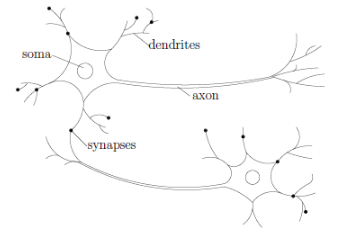
\includegraphics[scale=0.5]{neuron}
\caption{A neuron}
\label{f1}
\end{figure}

We mentioned weights $w_1, \ldots, w_m$ but did not reveal their role. Every
boolean expression requires a different neuron. Two neurons for different
boolean expressions with the same number of inputs differ in the weights 
attached to each input. `Training' an artificial neuron to decide a boolean
expression is the selection of weights so that the output is what we want.

\subsection{Mathematical notation}
Before proceeding further, we describe the mathematical notation used in
this is article. We denote by $\mathbb{R}$ the set of all real numbers. Vectors
are denoted with bold letters, for example $\vec{x} \in \mathbb{R}^d$ is a 
$d$-dimensional input vector. Matrices are denoted by sans serif letters. 
For example, $\mat{W}$ is a weight matrix.

\section{The Perceptron}\label{s2}
The American psychologist Frank Rosenblatt modified the McCulloch-Pitts neuron
allowing it take arbitrary inputs instead of boolean 
\cite{rosenblatt1958perceptron}. The function $\varphi$ in equation \eqref{s1e1}
was chosen to take the form of a step function
\begin{equation}\label{s2e1}
\theta(x) = \begin{cases}
0 \text{ if } x < 0 \\
1 \text{ if } x \ge 0.
\end{cases}
\end{equation}
The inputs $x_1, \ldots, x_m$ were augmented with a `bias' input $x_0$ which
was always $1$. The `weights' $w_1, \ldots, w_m$ were chosen in such a manner
that for most inputs $x_1, \ldots, x_m$, the perceptron produces the correct
output $y$. The algorithm to select the weights was also inspired by the way
biological neurons aid in human learning. The Canadian psychologist Donald Hebb
proposed \cite{hebb1949organization} that `neurons that fire together, wire
together', meaning that the connection between neurons grows if they are both
involved in a learning process. This suggested Rosenblatt that he should 
adjust the weights of the inputs based on the whether a given set of weights
produces correct output or not. Conversely, the weights are not adjusted if
they produce a correct output. We will demonstrate the perceptron learning
algorithm on the famous `iris' data set. The first step in data analysis is
always examining the data, which we do in the code below.
\begin{verbatim}
import numpy as np
import pandas as pd
import seaborn as sns
from sklearn import datasets
from sklearn.model_selection import train_test_split

df = sns.load_dataset("iris")
plot = sns.pairplot(df, hue="species")
plot.savefig('iris_pairplot.png')
\end{verbatim}

The pair plot of the four attributes of the data is
\begin{figure}[!ht]
\centering
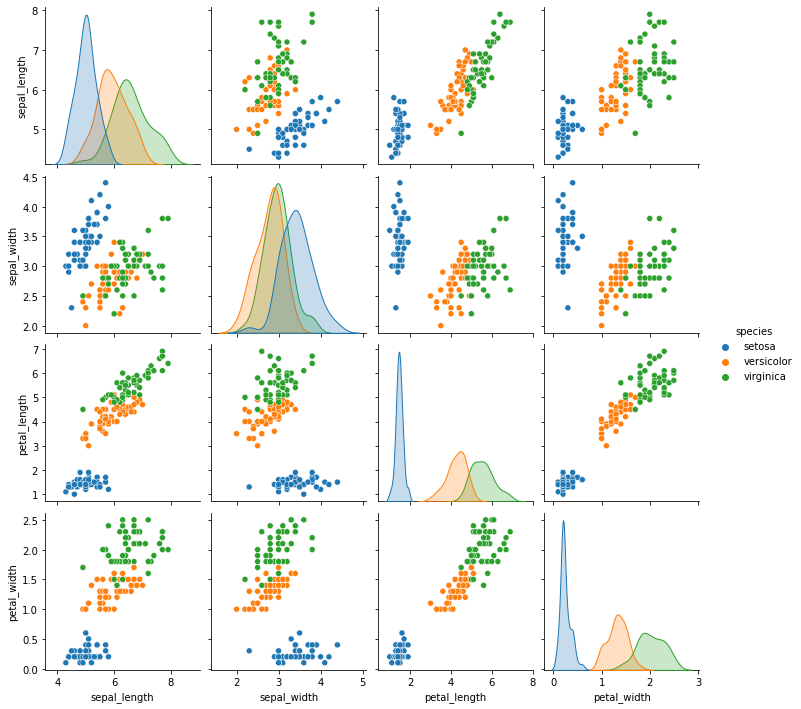
\includegraphics[scale=0.4]{iris}
\caption{Attributes of the iris dataset}
\label{f2}
\end{figure}

The pair plot in figure \ref{f2} suggests that petal width and petal length
are the best choice of attributes to tell the Setosa flowers from the other
two varieties. We add another attribute to the data set which takes a value
$1$ if the flower is Setosa and $-1$ if it is not. We then split the entire
data set into training and test data.

\begin{verbatim}
df['Class'] = np.where(df['species'] == 'setosa', 1, -1)
X_train, X_test, y_train, y_test = 
	train_test_split(df[['petal_length', 'petal_width']], \
                     df['Class'], \
                     test_size=1/3, \
                     random_state = 15081947)
\end{verbatim}

The next code listing has the core of the perceptron learning algorithm. We 
initialize weights to a small positive value. They are updated if for an 
observation the algorithm misclassifies it.
\begin{verbatim}
w = np.array([0.1, 0.1, 0.1]) 

def adjust_weights(X, y):
  global w
  z = X[0]*w[0] + X[1]*w[1] + w[2]
  if z > 0:
    y_hat = 1
  else:
    y_hat = -1
    
  w[0] += (y - y_hat) * X[0]
  w[1] += (y - y_hat) * X[1]
  w[2] += 1
\end{verbatim}

After running the algorithm on all observations in the training data set
we check its performance first on the training data set and then on the
test data set.
\begin{verbatim}
trn = pd.concat([X_train, y_train], axis=1)
tst = pd.concat([X_test, y_test], axis=1)
ignore = 
  trn.apply(lambda r: adjust_weights(r[['petal_length', 'petal_width']], \
            r['Class']), axis=1)

def classify(r):
  global w
  x = r[0]*w[0] + r[1]*w[1] + w[2]
  if x > 0:
    return 1
  else:
    return -1

trn_predict = trn.apply(lambda r: classify(r), axis=1)
tst_predict = tst.apply(lambda r: classify(r), axis=1)
\end{verbatim}

A cross-tabulation of the predicted and actual class shows that only $2$
out of $100$ training samples were misclassified. Repeating this step on
the test data shows that $3$ out of $50$ samples were misclassified. This 
error rate is not bad given the very simple algorithm we have used. We 
used this code to illustrate the essentials of the perceptron learning 
algorithm. A serious exercise in classification should use the perceptron
provided in the package \texttt{sklearn}. The code 
listing below shows that code.
\begin{verbatim}
from sklearn.linear_model import Perceptron

perceptron = Perceptron(random_state=26011950)
perceptron.fit(X_train, y_train)
y_pred = perceptron.predict(X_test)
\end{verbatim}
A cross-tabulation of the actual and the predicted class shows $100\%$
accuracy.

Equation \eqref{s2e1} is one choice of $\varphi$, the \emph{activation
function}. There are many others, some of which are shown in figure
\ref{f3}.
\begin{figure}[!ht]
\centering
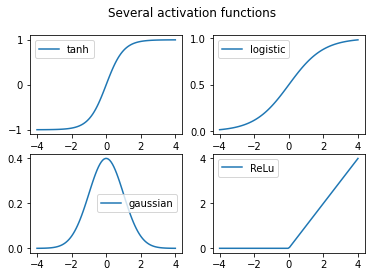
\includegraphics[scale=0.8]{activation}
\caption{Activation functions}
\label{f3}
\end{figure}

The perceptron was a sensation when it was first developed. It was 
implemented as hardware. However, it was soon discovered that it was
incapable of solving simple problems like the famous XOR problem. If
an output is an exclusive OR of its input then one cannot train a 
perceptron to evaluate it. In fact, it was soon shown that a perceptron 
functions best when there is a linear boundary separating the various
classes of inputs. Several problems do not have such a boundary and
therefore they are outside the purview of a perceptron.

\section{Multi-level Perceptrons}\label{s3}
Some limitations of a single perceptron can be overcome by building a
network of perceptrons. The term `multi-level perceptron' is network of
perceptrons with one layer taking inputs, another one producing the output
and one or more intermediate layers. It does not mean a perceptron with
multiple layers. It is a stack of perceptrons. Although the idea of a 
network of neurons was explored since the times of McCulloch and Pitts model
there is no algorithm to train the networks. In this section we will 
describe feed-forward multi-level perceptrons. The adjective `feed-forward'
means that the output of a neuron is not fed as an input to itself or
another neuron of a previous layer.

We summarize the behavior of a single perceptron in the following
equations \cite{bishop1994neural}.
\begin{eqnarray}
\sum_{i=0}^d w_i x_i &=& a \label{s3e1} \\
g(a) &=& z \label{s3e2},
\end{eqnarray}
where the input $x_0$ is always $1$, there are $d$ other inputs $x_1, 
\ldots, x_d$ and $g$ is a suitable activation function. We consider a
multi-layer perceptron with just a single hidden layer with a topology
shown in figure \ref{f4}.
\begin{figure}[!ht]
\centering
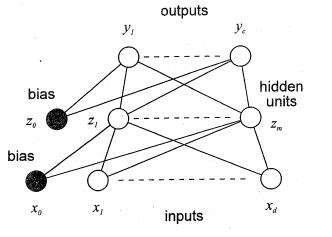
\includegraphics[scale=0.8]{mlp}
\caption{Multi-layer perceptron (from ref. \cite{bishop1994neural})}
\label{f4}
\end{figure}
There are $d + 1$ inputs and $m$ outputs in the first layer. The $m$ 
outputs are the inputs to the $m$ neurons in the second layer. The output
of every neuron in the first layer is fed as an input to the second layer.
Therefore there are $(d + 1) \times m$ weights, denoted by $w_{ij}^{(1)}$ with
$i$ ranging from $0$ to $d$ and $j$ ranging from $1$ to $m$. Using the 
notations of equations \eqref{s3e1} and \eqref{s3e2}, we can write
\begin{equation}\label{s3e3}
z_j = g_1\left(\sum_{i=0}^d w_{ji}^{(1)}x_i\right).
\end{equation}
The $z_j$ along with $z_0 = 1$ form the inputs to the second layer so that 
the final output is
\begin{equation}\label{s3e4}
y_k = g_2\left(\sum_{j=0}^m w^{(2)}_{jk} g_1\left(\sum_{i=0}^d w^{(1)}_{ij}x_i
\right)\right),
\end{equation}
The activation functions $g_1$ and $g_2$ in equations \eqref{s3e3} and 
\eqref{s3e4} may be same or they could differ. If they are linear functions
then the network is no different from matrix multiplication. In they are
non-linear then the network can represent quite complicated functions. It can
be shown that if $m$ is sufficiently large then the network of figure \ref{f4}
can represent any continuous function defined over a finite range of its
domain, to arbitrary accuracy \cite{bishop1994neural}. When a nulti-layer
perceptron is used for classification it is common to have $g_2$ to be the
softmax function so that one can interpret the outputs $y_1, \ldots, y_c$ as
the probability of membership in classes $1, \ldots, c$.

We saw several activation functions in figure \ref{f3}. We can use all of
these except the step function. The algorithm to train multi-layer preceptron 
requires finding the 
derivative of the activation function. The last one, namely, $g(x)=\max(0, x)$ 
is not differentiable at the origin. However, that is usually not a problem. 
The hyperbolic tangent and the logistic functions are especially favored because
their derivatives can be expressed in terms of themselves. From a numerical
perspective, computing the derivative at a certain value is easy if we have
computed the function at the same value. This follows from the fact that if
$g(x) = \tanh(x)$ then $g^\prime(x) = 1 + (g(x))^2$ and if $g(x) =
(1+e^{-x})^{-1}$ then $g^\prime(x) = g(x)(1 - g(x))$.

Training the network means selecting the `best' choices of the weights 
$w^{(1)}_{ij}$ and $w^{(2)}_{jk}$ such that the values of the output $y_k$ 
are as close to the unknown function as possible. If we are given that an
input $\vec{x}^q = (x_1^q, \ldots, x_d^q)$ corresponds to a value $\vec{t}^q
= (t_1^q, \ldots, t_c^q$ (refer to figure \ref{f4}) then the error function
for this input is
\begin{equation}\label{s3e5}
E = \frac{1}{2}\sum_{q=1}^n ||\vec{t}^q - \vec{y}^q||^2,
\end{equation}
where $\vec{y}^q = (y_1^q, \ldots, y_c^q)$ is the output of the network. The
quantity $E$ is a function of the weights $w^{(1)}_{ij}$ and $w^{(2)}_{jk}$.
Training the network is thus finding the minimum of the function $E$. In 
general, $E$ can have several minima and the challenge of a network training
algorithm is the find the least among all the minima. This choice of the
minimum is called the \emph{global} minimum. There are several optimization
algorithms to compute extrema of functions of several variables. In the case
of the error function of \eqref{s3e5}, where $\vec{y}^q$ is the output of a
multi-layer perceptron, an efficient algorithm is based on \emph{error
backpropagation} \cite{rumelhart1985learning}. For each pair $(\vec{x}^q, 
\vec{t}^q)$, the algorithm first computes the error $\vec{t}^q - \vec{y}^q$
and then it attributes a portion of the error to each neuron of the previous
layers, reaching all the way down to the input layer. It then adjusts the 
weights starting from the input layer al the way up to the output layer to 
minimize the error. In modern terms, it can be described as a gradient descent 
with an auto-diff \cite{geron2019hands}.

We will illustrate classification using the multi-layer perceptron in the
code snippets below. The first among these imports the necessary packages.
\begin{verbatim}
import numpy as np
import pandas as pd
import seaborn as sns
import matplotlib.pyplot as plt
from sklearn import datasets
from sklearn.model_selection import train_test_split
from sklearn.neural_network import MLPClassifier
from sklearn import preprocessing
from sklearn.metrics import average_precision_score, confusion_matrix
from sklearn.metrics import accuracy_score, classification_report
from sklearn.metrics import plot_confusion_matrix
\end{verbatim}

We then load the data set and encode the class as a number.
\begin{verbatim}
df = sns.load_dataset("iris")
encoder = preprocessing.LabelEncoder()
df['species_class'] = encoder.fit_transform(df['species'])
\end{verbatim}

After splitting the data set as
\begin{verbatim}
X_train, X_test, y_train, y_test = 
	train_test_split(df[['petal_length', 'petal_width']], \
                     df['species_class'], \
                     test_size=1/3, \
                     random_state = 15081947)
\end{verbatim}
we train a multi-layer perceptron classifier 
\begin{verbatim}
clf_0 = MLPClassifier(hidden_layer_sizes=(3, 3), \
                     random_state=15081947, \
                     solver='lbfgs', \
                     alpha=1e-5)
clf_0.fit(X_train, y_train)
\end{verbatim}
and use it on the test data
\begin{verbatim}
y_pred = clf_0.predict(X_test)
\end{verbatim}
Finally, we check the quality of our prediction.
\begin{verbatim}
accuracy_score(y_test, y_pred)

# Print the classification report.
y_test_orig = encoder.inverse_transform(y_test)
y_pred_orig = encoder.inverse_transform(y_pred)
print(classification_report(y_test_orig, y_pred_orig, digits=2))

# Print the confusion matrix.
conf_mat = confusion_matrix(y_test_orig, y_pred_orig)
ctypes = ['setosa ', 'versicolor', 'virginica']
df_conf_mat = pd.DataFrame(conf_mat, index = ctypes, columns = ctypes)
plt.figure(figsize = (10,7))
ignore = sns.heatmap(df_conf_mat, annot=True, cmap='Blues', fmt='g')
\end{verbatim}

\section{Recurrent Neural Networks}\label{s4}
Although a multi-layer perceptron has several layers of neurons, information
always flows from the input to the output. The output of every layer of 
neurons is either fed as the input to the next layer above it or it is the
final output. Such networks are called \emph{feed-forward} networks. When the
`current' output of a neuron is fed as its `next' input then the neuron 
acquires two characteristics
\begin{itemize}
\item The `current' state of the neuron becomes a function of all its `previous'
states and 
\item There is a sense of `time' introduced in the operation, as is evident
in the use of the terms `previous', `current' and `next'.
\end{itemize}
Such a neuron is called a recurrent neuron and a network of such neurons is
called a recurrent neural network (RNN). Several tasks in artificial 
intelligence require an algorithm to process a long sequence of input values
and its behavior depends, in principle, on all the values it was fed. For
example, the sentiment conveyed in a paragraph of natural language cannot be
accurately gauged unless we read it \emph{in toto}. It may start with a several
sentences indicating displeasure but end with a statement indicating 
satisfaction at an overall level. Or it could be the other way round. Certain
other signals may have a long series of uninteresting values punctuated by
extreme values which have a disproportionate influence on the course of the 
series. For example, we could be tracking price of a commodity that stays
within narrow bounds for a very long time but takes a drastically different
value once in a while. If we were to examine the time series of prices we
might want to model the fact that the `next' value in the series depends on
the extreme values seen in the past. Problems like these find a natural
expression in recurrent neural networks.

Let us consider a single neuron that takes an input $\vec{x} \in \mathbb{R}^d$
and produces an output $\vec{y} \in \mathbb{R}^m$. The $d$ inputs are
associated with an equal number of weights $w^{(x)}_i$, $i = 1, \ldots, d$. If
we feed the output $\vec{y}$ to the input, then we will need an additional
$m$ weights $w^{(y)}_i$, $i = 1, \ldots, m$. If we denote the input at step 
$t$ as $\vec{x}_t$ and the corresponding output as $\vec{y}_t$ then we can
express the recurrent neuron mathematically as
\begin{equation}\label{s4e1}
\vec{y}_t = g\left(\vec{x}_t\cdot\vec{w}^x+\vec{y}_{t-1}\cdot\vec{w}^y\right),
\end{equation}
where the $\cdot$ operation between the vectors represents their inner product
and $g$ is an activation function. Note that $\vec{w}^x \in \mathbb{R}^d$ and
$\vec{w}^y \in \mathbb{R}^m$. 
Not that the output at step $t$ depends on the input at step $t$ and the output
at the \emph{previous} step $t-1$. When we begin the computations, we do not
have the \emph{previous} value of $\vec{y}$. As a result, we must mention
it as a part of the network's specification. If the bias term is not a part
of the input then we include it separately and write equation \eqref{s4e1}
as
\begin{equation}\label{s4e2}
\vec{y}_t=g\left(\vec{x}_t\cdot\vec{w}^x+\vec{y}_{t-1}\cdot\vec{w}^y+b\right),
\end{equation}
The networks of equations \eqref{s4e1} and \eqref{s4e2} fed their output
as the input of the next step. This might not always be the case. Instead, a
neuron might feed a different set of numbers, collected as a vector $\vec{h}$,
to the input. In this case, $\vec{h}$ is called a \emph{hidden state} and it
differs from the cells output $\vec{y}$. Equation \eqref{s4e2} is modified
to
\begin{equation}\label{s4e3}
\vec{y}_t=g\left(\vec{x}_t\cdot\vec{w}^x+\vec{h}_{t-1}\cdot\vec{w}^h+b\right),
\end{equation}
The fact that a recurrent neuron is fed a sequence of inputs and that it 
produces a sequence of outputs leads to several possibilities of interpreting
the inputs and the outputs.
\begin{itemize}
\item A recurrent neuron may be fed a sequence $\vec{x}_0, \ldots, \vec{x}_t$
and we may read off its output $\vec{y}_m, \ldots, \vec{y}_{m+t}$. Thus, 
we are trying to predict the value of the time series $m$ steps ahead. Such
a neuron is called a sequence-to-sequence neuron.
\item If we feed the neuron a sequence $\vec{x}_0, \ldots, \vec{x}_t$ and
consider just $\vec{y}_{t+1}$ then we have a sequence-to-vector neuron. The 
input could be prices of an asset over a certain period until `now' and we
try to predict what it will be `next'.
\item If the input to the neuron is the sequence $\vec{x}_0, 0, \ldots, 0$,
where $0$ is repeated $t - 1$ times and we consider the output $\vec{y}_1,
\ldots, \vec{y}_{t+1}$ then we are treating the neuron like a differential
equation. Given an initial value, we compute its entire trajectory in the
future. Such a neuron is called a vector-to-sequence neuron.
\item Alternatively, we feed the neuron a sequence $\vec{x}_0, \ldots, 
\vec{x}_m$ followed by $n$ zeros and read the output $\vec{y}_{m+1}, \ldots,
\vec{y}_{m+n}$. Such a neuron is called an encoder-decoder because one can
interpret its operation as an encoding of an input sequence in the form of
an output sequence. An example of such a usage could be reading $m$ words of
one natural language and producing $n$ words of another natural language. One
often cannot correctly translate a text without reading a substantial portion
of it.
\end{itemize}

One can easily adapt the back propagation algorithm to train a recurrent
neuron. Instead of considering a single neuron working across time, one can
mentally imagnine $n$ copies of the neuron at times $0, \ldots, n-1$, each
with the appropriate inputs, hidden states and outputs. We then compare the
outputs with the desired outputs and adjust the weights to minimize the
difference between them. This modification is called \emph{back propagation
through time}. Recall that the error in the network, a measure of the 
difference between the predicted and actual output, is a function of the 
weights. Minimzing the error is then finding a minimum of a function of
weights. The back propagation algorithm finds the minimum by computing the
derivative of the error. When a function depends on more than one variable, it
does not have a single derivative. Rather its derivative depends on the 
direction in space along with we are computing it. In fact, a derivative in
the case of a function of several variables is often called the directional
derivative. Among all directional derivatives, the one that has the maximum
magnitude is called the gradient of the function. In the case of the function
defined in equation \eqref{s3e5} it is denoted by $\nabla E$. Although $E$
is a scalar quantity, $\nabla E$ is a vector. The back propagation algorithm 
functions well as long $\nabla E$ is not zero or does not have a very large
magnitude. These two situations are termed as `vanishing' and `exploding'
gradients. Since $\nabla E$ also depends on the activation function, one can
sometimes mitigate the problem of vanishing and exploding gradients by choosing
the appropriate activation function. A popular choice is $g(x) = \max(0, x)$,
also called ReLU. Since these problems arise in back-propagation algorithm of
training multi-layer perceptrons, they also plague the training of recurrent
neural networks using back-propagation in time algorithm. In the case of
RNNs one way to prevent them is to trunctate the number of steps in the 
history one uses to adjust the weights. This is called truncated back-
propagation in time \cite{geron2019hands}.

Vanishing and exploding gradients is not the only challenge in training RNNs. 
We mentioned previously that many times distant history of the inputs is quite
significant to get correct outputs. However, it is never clear how much distant
in the past one must look to ensure correct output. Over a long sequence of
steps the memory of the earliest inputs gets faded and stops affecting the 
output in any significant manner. This is definitely a problem when it is 
important to remember the `significant' features discovered early on. This
shortcoming is overcome with a long short-term memory (LSTM) cell 
\cite{hochreiter1997long}. 

An LSTM cell has two hidden states $\vec{h}_t$ and $\vec{c}_t$ used to 
store information about the `short-term' and the `long-term'. Its input is
denoted by $\vec{x}_t$ and output as $\vec{y}_t$. When looked at this level,
the only difference between the plain version of recurrent neuron of equation
\eqref{s4e3} and this one is the existence of yet another `hidden state' in the
form of $\vec{c}_t$. In order to compute the output at step (or time) $t$, the
LSTM cell needs $\vec{x}_t, \vec{h}_{t-1}$ and $\vec{c}_{t-1}$. It computes
the output and updates its hidden states as follows;
\begin{itemize}
\item The input $\vec{x}_t$ and the short-term hidden state $\vec{h}_{t-1}$ are
used to determine which part of the input should be added to the long-term
hidden state. This is done by computing
\begin{equation}\label{s4e4}
\vec{i}_t = \sigma\left(\mat{W}_{xi}\vec{x}_t + \mat{W}_{hi}\vec{h}_{t-1} + 
\vec{b}_i\right),
\end{equation}
where $\mat{W}_{xi}$ and $\mat{W}_{hi}$ are weight matrices and $\vec{b}_i$ is
the bias and $\sigma$ denotes the logistic function.
\item The input $\vec{x}_t$ and the short-term hidden state $\vec{h}_{t-1}$ are
used to determine which part of the input should be erased the long-term
hidden state. This is done by computing
\begin{equation}\label{s4e5}
\vec{f}_t = \sigma\left(\mat{W}_{xf}\vec{x}_t + \mat{W}_{hf}\vec{h}_{t-1} + 
\vec{b}_f\right),
\end{equation}
where $\mat{W}_{xf}$ and $\mat{W}_{hf}$ are weight matrices and $\vec{b}_f$ is
the bias.
\item The input $\vec{x}_t$ and the short-term hidden state $\vec{h}_{t-1}$ are
used to determine which part of the long-term hidden state should be read and
used to get the final output. This is done by computing
\begin{equation}\label{s4e6}
\vec{o}_t = \sigma\left(\mat{W}_{xo}\vec{x}_t + \mat{W}_{ho}\vec{h}_{t-1} + 
\vec{b}_o\right),
\end{equation}
where $\mat{W}_{xo}$ and $\mat{W}_{ho}$ are weight matrices and $\vec{b}_o$ is
the bias.
\item We next compute $\vec{g}_t$ as
\begin{equation}\label{s4e7}
\vec{g}_t = \tanh\left(\mat{W}_{xg}\vec{x}_t + \mat{W}_{hg}\vec{h}_{t-1} + 
\vec{b}_g\right),
\end{equation}

Note that the functional form of the arguments of equations \eqref{s4e4}, 
\eqref{s4e5}, \eqref{s4e6} and \eqref{s4e7} is identical. Further, the function
in the first three equation is identical. The vectors $\vec{i}_t, \vec{f}_t$, 
$\vec{o}_t$ and $\vec{g}_t$ are used to compute the `next' state of the cell 
and its output.
\item The long-term state is updated as
\begin{equation}\label{s4e8}
\vec{c}_t = \vec{f}_t \circ \vec{c}_{t-1} + \vec{i}_t \circ \vec{g}_t,
\end{equation}
where $\circ$ denotes the Hadamard product. 
\item The short-term state and the output are updated as
\begin{eqnarray}
\vec{h}_t &=& \vec{o}_t \circ \tanh(\vec{c}_t) \label{s4e9} \\
\vec{y}_t &=& \vec{o}_t \circ \tanh(\vec{c}_t) \label{s4e10} 
\end{eqnarray}
Note that the two values are identical.
\end{itemize}
It is customary to call $\vec{i}_t$ the input gate, $\vec{o}_t$ the output gate
(not to be confused with \emph{the} cell output $\vec{y}_t$) and $\vec{f}_t$
the forget gate. This also explains the choice of variables used to denote them.
Equation \eqref{s4e8} is interpreted as `forgeting' some long term memory
and `updating' it with the current state. The final output is produced from
$\vec{c}_t$ and the `output gate' $\vec{o}_t$. Figure \ref{f5} shows an
LSTM cell. FC stands for fully connected unit in both figures \ref{f5} and 
\ref{f6}.
\begin{figure}
\centering
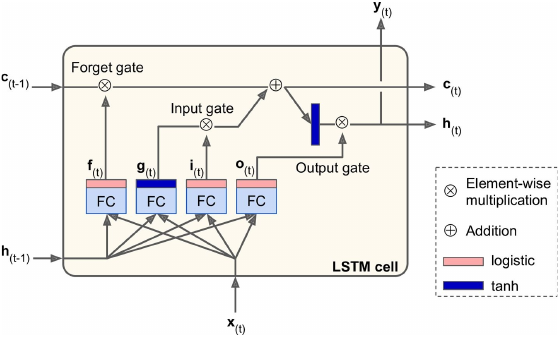
\includegraphics[scale=0.5]{lstm}
\caption{LSTM from \cite{geron2019hands}}\label{f5}
\end{figure}

A simplification of the LSTM cell was achieved by the gated recurrent unit
(GRU) \cite{cho2014learning}. It keeps just one hidden state $\vec{h}_t$ and
one of the pair $\vec{i}_t$ and $\vec{f}_t$, which it calls $\vec{z}_t$. A
new gate $\vec{r}_t$ is added to combine the current input to the hidden state
computed in the previous step. A GRU can be expressed as
\begin{eqnarray}
\vec{z}_t&=&\sigma\left(\mat{W}_{xz}\vec{x}_t+\mat{W}_{hz}\vec{h}_{t-1}\right) 
\label{s4e11} \\
\vec{r}_t&=&\sigma\left(\mat{W}_{xr}\vec{x}_t+\mat{W}_{hr}\vec{h}_{t-1}\right) 
\label{s4e12} \\
\vec{g}_t&=&\tanh\left(\mat{W}_{xg}\vec{x}_t+\mat{W}_{hg}(\vec{r}_t\circ
\vec{h}_{t-1})\right) \label{s4e13} \\
\vec{h}_t&=&(1 - \vec{z}_t)\circ\vec{h}_{t-1} + \vec{z}_t\circ\vec{g}_t
\label{s4e14} \\
\vec{y}_t&=&(1 - \vec{z}_t)\circ\vec{h}_{t-1} + \vec{z}_t\circ\vec{g}_t
\label{s4e15}
\end{eqnarray}

\begin{figure}
\centering
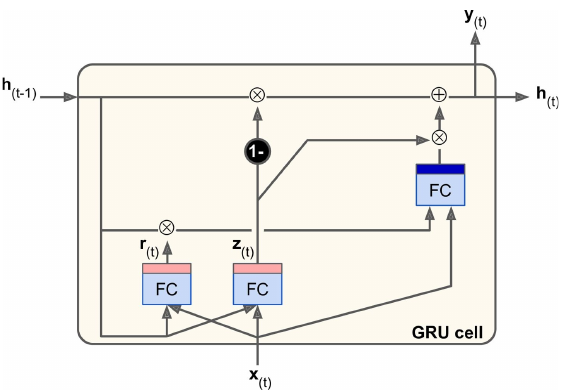
\includegraphics[scale=0.5]{gru}
\caption{A gated recurrent unit from \cite{geron2019hands}}\label{f6}
\end{figure}
Once again the output and the hidden state are identical. There are no bias
vectors. The input $\vec{x}_t$ is combined with the hidden state $\vec{h}_t$
in two stages, equations \eqref{s4e12} and \eqref{s4e13}. LTSM and GRU are the
most dominant architectures of recurrent neural networks used currently. 

We can treat a GRU as a black box and represent equations \eqref{s4e11} to
\eqref{s4e15} as just
\begin{equation}\label{s4e16}
\vec{y}_t = \vec{h}_t = f(\vec{h}_{t-1}, \vec{x}_t, \theta),
\end{equation}
where $\theta$ denote all the weights of the GRU. The learning of a GRU can be 
interpreted as learning the conditional probability distribution 
$p(\vec{x}_t | \vec{x}_{t-1}, \ldots, \vec{x}_1)$. For a $d$-dimensional input, 
we can write this vector conditional probability as
\[
\prod_{i=1}^d p(x^i_t | x^i_{t-1}, \ldots, x^i_1).
\]
When used as an encoder-decoder, the training of the GRU can be viewed as the
maximization of the conditional log-likelihood
\begin{equation}\label{s4e17}
L(\theta) = \frac{1}{N}\sum_{n=1}^N\log p_\theta(\vec{y}_n|\vec{x}_n),
\end{equation}
where $\vec{x}_n$ and $\vec{y}_n$ are the input and output vectors at time $n$
and they need not be of the same dimensions. $\theta$ are all the parameters 
of the GRU, that is, the all the weight matrices of equations \eqref{s4e11}
to \eqref{s4e15}. In the encoder-decoder model, we can interpret the 
mechanism of producing the output as a two stage process. The inputs are
converted into a \emph{context vector} which is then transformed into the final
output. A limitation of the GRU architecture is the limited length of its
context vector. In the context of natural language processing it shows up as
the inability of a GRU to remember long sentences. The attention layer tries
to overcome this limitation by allowing the model to automatically search for
portions of input that it feels are most relevant for producing the correct
output \cite{bahdanau2014neural}. The attention layer is not important for 
natural language processing alone. When neural networks are used for image
recognition, they have to `remember' the most distingushing features of the
image while scanning the rest of it. For example, when scanning the picture of
the tiger in a dark surrounding, the most important part to `pay attention' to
is its shining eyes. Another example is shown in figure 1 of reference 
\cite{weng2018attention}.

Focusing our attention on the problem of neural machine translation, one way
to build an attention layer is to have two hidden states $\vec{f}_t$ and 
$\vec{b}_t$, called forward and backward hidden states. The encoder's hidden
state is just a concatenation of the two. The decoder has a different hidden
state $\vec{s}_t = u(\vec{s}_{t-1}, \vec{y}_{t-1}, \vec{c}_t)$, where 
$\vec{c}_t$ is the context vector. It is the weighted sum of the encoder's
hidden state. The weights are the alignment scores $\alpha_{ij}$. The number
$\alpha_{ij}$ is a measure of how well the input at position $i$ matches the
output at position $j$. The alignment scores permit the network with an 
attention layer to remember distant parts of input while still keeping the
context vector of a limited size. We refer to the web article 
\cite{weng2018attention} for an excellent account of the attention layer 
applied to problems in image processing and natural language translation.
\bibliographystyle{plain}
\bibliography{nn}
\end{document}
